\chapter{Multiple Pattern Matching}

\section{Multiple Pattern Matching Problem}

Consider a scenario where instead of searching for a single pattern, we need to find multiple patterns simultaneously within a text.

Given a text $T$ of length $n$ and a collection of $k$ patterns $P_1, \dots, P_k$ with respective lengths $m_1, \dots, m_k$, we want to find all occurrences of any pattern within the text.

A naive approach would be to apply the KMP algorithm $k$ times, once for each pattern. This would yield a computational complexity of $O(\sum_{i=1}^k m_i + k \times n)$, where the first term accounts for preprocessing all patterns and the second term represents $k$ separate scans of the text. Our goal is to reduce this complexity to $O(\sum_{i=1}^k m_i + n)$, eliminating the factor of $k$ in the text scanning phase. This improvement can be achieved by preprocessing the text $T$ instead of the individual patterns $P_i$, allowing us to search for all patterns simultaneously in a single pass.

\subsubsection{Trie Data Structure}

To efficiently handle multiple patterns, we introduce the concept of a \textbf{trie} (prefix tree). A trie is a specialized tree data structure that serves as an efficient dictionary for string storage and retrieval.

Formally, a trie is a rooted tree with the following properties:
\begin{itemize}
    \item \textbf{Edge labeling:} Each edge is labeled with a letter from alphabet $\Sigma$
    \item \textbf{Unique branching:} No two edges branching from the same node are labeled with the same letter
    \item \textbf{String representation:} Each path from root to leaf represents a string in our collection
\end{itemize}

Tries can compactly represent sets of strings and function as a type of dictionary data structure. For a collection of strings $T_1, \dots, T_k$, the maximum number of nodes in the corresponding trie is $\Theta(\sum_{i=1}^k |T_i|)$, which equals the total number of characters across all strings.

\begin{exampleblock}[Trie]

\begin{minipage}{0.7\textwidth}
Let's define our set of strings as:
\vspace{0.4cm}
$$
\qquad R = \{\text{ana}, \text{ann}, \text{anna}, \text{anne}\}
$$

The trie structure shown on the right represents $Trie(R)$.

It demonstrates how all strings in $R$ begin with the common prefix \plaintt{an} before diverging into their distinct suffixes. The structure maps each string in $R$ to a unique path from the root to a leaf.

\vspace{0.4em}

The trie's efficiency comes from its ability to store shared prefixes only once, eliminating redundancy. This compression allows us to search for all patterns simultaneously by following the text's characters through the tree structure.


\end{minipage}%
\begin{minipage}{0.3\textwidth}
    \centering
        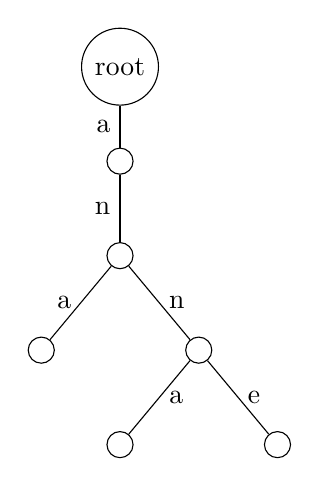
\begin{tikzpicture}[scale=0.8, level distance=1.5cm, sibling distance=2.5cm]
        
        \node[circle, draw] {root} 
            child {node[circle, draw] {}
                child {node[circle, draw] {}
                    child {node[circle, draw] {}
                        edge from parent node[left] {a} 
                    }
                    child {node[circle, draw] {}
                        child {node[circle, draw] {}
                            edge from parent node[right] {a}}
                        child {node[circle, draw] {}
                            edge from parent node[right] {e}}
                        edge from parent node[right] {n}
                    }
                    edge from parent node[left] {n}
                }
                edge from parent node[left] {a} 
            };
        \end{tikzpicture}
    \end{minipage}
\end{exampleblock}
    
A \textbf{compacted trie} is a rooted tree whose edges are labeled by strings over alphabet $\Sigma$ such that no two edges branching from the same node are labeled starting by the same letter. All nodes but the leaves have at least two children. The maximum number of nodes a compacted trie can have is $2k$, so $\Theta(k)$, where $k$ is the number of words in the set.
    
\begin{exampleblock}[Compacted Tries]
    
    \begin{minipage}{0.7\textwidth}
    Let's define our set of strings as
    \vspace{0.4em}
    $$
    \qquad T = \{\text{ana}, \text{ann}, \text{anna}, \text{anne}\}
    $$
    
    Then, its compacted trie would be the one in the right. It demonstrates how all strings in $T$ share the common prefix \plaintt{an} before diverging into their distinct suffixes.
    
    Also in this case, he structure maps each string in $T$ to a unique path from the root to a leaf.
    

    \end{minipage}%
    \begin{minipage}{0.3\textwidth}
        \centering
        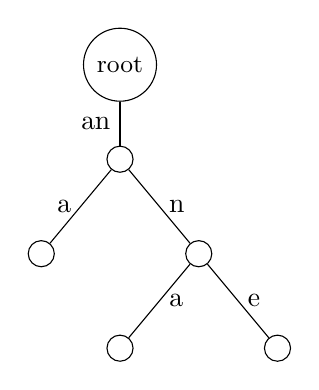
\begin{tikzpicture}[scale=0.8, level distance=1.5cm, sibling distance=2.5cm]
        
        \node[circle, draw] {\small root} 
            child {node[circle, draw] {}
                child {node[circle, draw] {}
                    edge from parent node[left] {a} 
                }
                child {node[circle, draw] {}
                    child {node[circle, draw] {}
                        edge from parent node[right] {a}}
                    child {node[circle, draw] {}
                        edge from parent node[right] {e}}
                    edge from parent node[right] {n}
                }
                edge from parent node[left] {an}
            };
        \end{tikzpicture}
    \end{minipage}
    
\end{exampleblock}
        
\section{Suffix trees}

\subsection{Suffix Tree}

A \textbf{suffix tree} represents a string $T$ as a compacted trie containing all its suffixes. To ensure that each suffix terminates at a leaf node, we append a special end marker $\$$ (where $\$ \notin \Sigma$) to $T$. The suffix tree is then constructed from the extended string $T\$$. This modification ensures that there are no suffixes that are prefixes of other suffixes, which could otherwise appear in an internal node.

\begin{exampleblock}[Suffix Trees]
    
    Let's define $T$ as:

    \vspace{-1em}

        \begin{table}[H]
        \small
        \centering
        \begin{tabular}{cccccccc}
            \textbf{T} & b & a & n & a & n & a & $\$$\\
            \textbf{Pos} & 1 & 2 & 3 & 4 & 5 & 6 & 7\\
        \end{tabular}
        \label{tab:my_label}
    \end{table}

    \vspace{-1.2em}

    where $\$ \notin \Sigma$. Then, we can define the list of suffixes of $T$ as:

    \vspace{-0.6em}
    
    \begin{table}[H]
        \small
        \centering
        \begin{tabular}{ccccccc}
            \multicolumn{7}{c}{\textbf{Suffixes}}\\
            b & a & n & a & n & a & $\$$\\
                & a & n & a & n & a & $\$$\\
                &  & n & a & n & a & $\$$\\
                &  &  & a & n & a & $\$$\\
                &  &  &  & n & a & $\$$\\
                &  &  &  &  & a & $\$$\\
                &  &  &  &  &  & $\$$\\
        \end{tabular}
        \label{tab:my_label}
    \end{table}

    \vspace{-1.2em}
    
    Then, its suffix tree would be:

    \begin{center}
        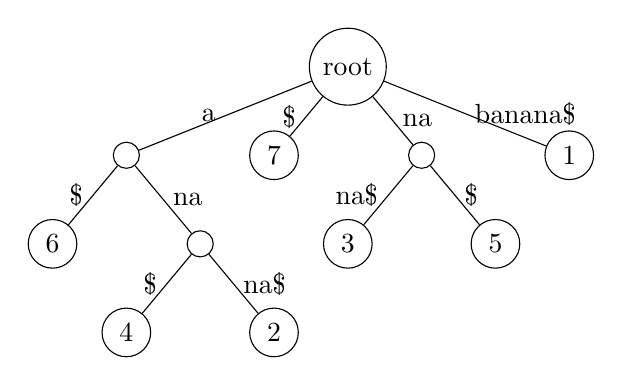
\begin{tikzpicture}[scale=0.75, level distance=1.5cm, sibling distance=2.5cm]
        
        \node[circle, draw] {root} 
            child {node[circle, draw] {}
                child {node[circle, draw] {6}
                    edge from parent node[left] {\$}} 
                child {node[circle, draw] {}
                    child {node[circle, draw] {4}
                        edge from parent node[left] {\$}} 
                    child {node[circle, draw] {2}
                        edge from parent node[right] {na\$}} 
                    edge from parent node[right] {na}} 
                edge from parent node[left] {a}}
            child {node[circle, draw] {7}
                edge from parent node[left] {\$}} 
            child {node[circle, draw] {}
                child {node[circle, draw] {3}
                    edge from parent node[left] {na\$}} 
                child {node[circle, draw] {5}
                    edge from parent node[right] {\$}} 
                edge from parent node[right] {na}} 
            child {node[circle, draw] {1}
                edge from parent node[right] {banana\$}} ;
        \end{tikzpicture}
    \end{center}  

    where the labels of the leaves correspond to starting positions of suffixes in $T$.
\end{exampleblock}

\begin{observationblock}
    The number in each leaf represents the starting position of the suffix in the string.
\end{observationblock}

To search for a pattern $P$ in the suffix tree $ST$ of $T$:

\begin{itemize}
    \item Follow the path in $ST$ that spells out the letters of $P$.
    \begin{itemize}
        \item If you can spell the entire $P$, then all occurrences of $P$ in $T$ correspond to the leaf IDs below.
        \item If you cannot spell all of $P$, then $P$ does not occur in $T$.
    \end{itemize}
\end{itemize}

For a string $T$ of length $n$, the compacted suffix tree exhibits remarkable space efficiency with $O(n)$ nodes and $O(n)$ edges. While a naive representation would require $O(n^2)$ space due to potentially storing full substrings as edge labels.

Recalling that every substring of $T$ is a prefix of some suffix of $T$, meaning each substring maps to a unique path from the root in the suffix tree. This elegant property allows us to represent each edge label as a simple interval of positions over $T$, requiring only $O(1)$ space per edge. Since the tree contains $O(n)$ edges, this compact representation reduces the total space complexity to $O(n)$, making suffix trees both powerful and practical for large-scale string processing.

\begin{exampleblock}

Let's define $T$ as

\vspace{-1em}

\begin{table}[H]
    \small
    \centering
    \begin{tabular}{cccccccc}
        \textbf{T} & b & a & n & a & n & a & $\$$\\
        \textbf{Pos} & 1 & 2 & 3 & 4 & 5 & 6 & 7\\
    \end{tabular}
    \label{tab:my_label}
\end{table}

\vspace{-1em}

Then, its new suffix tree would be

\color{black}
\begin{center}
    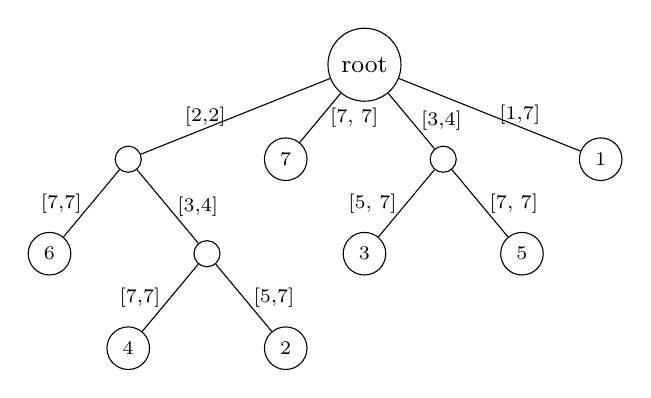
\begin{tikzpicture}[scale=0.8, level distance=1.5cm, sibling distance=2.5cm]
    
    \node[circle, draw] {\small root} 
        child {node[circle, draw] {}
            child {node[circle, draw] {\scriptsize 6}
                edge from parent node[left] {\scriptsize [7,7]}} 
            child {node[circle, draw] {}
                child {node[circle, draw] {\scriptsize 4}
                    edge from parent node[left] {\scriptsize [7,7]}} 
                child {node[circle, draw] {\scriptsize 2}
                    edge from parent node[right] {\scriptsize [5,7]}} 
                edge from parent node[right] {\scriptsize [3,4]}} 
            edge from parent node[left] {\scriptsize [2,2]}}
        child {node[circle, draw] {\scriptsize 7}
            edge from parent node[right] {\scriptsize [7, 7]}} 
        child {node[circle, draw] {}
            child {node[circle, draw] {\scriptsize 3}
                edge from parent node[left] {\scriptsize [5, 7]}} 
            child {node[circle, draw] {\scriptsize 5}
                edge from parent node[right] {\scriptsize [7, 7]}} 
            edge from parent node[right] {\scriptsize [3,4]}} 
        child {node[circle, draw] {\scriptsize 1}
            edge from parent node[right] {\scriptsize [1,7]}} ;
    \end{tikzpicture}
    \end{center}
    Note that each interval represents any occurrence in the string of its corresponding substring.
\end{exampleblock}


\subsubsection{Suffix Tree Construction}

The steps to build the suffix tree are represented in the following algorithm.

\vspace{-0.5em}

\begin{algorithm}[H]
\caption{Naïve\_construct\_ST(T)}
\label{alg:ann}

\Input{A string $T$ of length $n$}
\Output{The suffix tree $ST$ of $T$}

\hl

\begin{algorithmic}[1]
    \State $ST \gets \emptyset$
    \For{$i = 1$ to $i=n+1$}
        \State Spell $T[i, \dots, n+1]$ from the root of ST until arriving at a node $u$
        \State Branch from $u$ and add an edge with the remaining part of $T[i, ..., n+1]$
    \EndFor
    \State \Return ST
\end{algorithmic}
\end{algorithm}

\vspace{-1.3em}

The worst case is when the text is a single character repeated $n$ times, then the complexity of this algorithm is $O(n^2)$.

\subsubsection{Suffix Tree Representations}

There are different ways of representing a suffix tree, each one with its advantages and drawbacks.


\begin{table}[H]
    \centering
    \renewcommand{\arraystretch}{1.25}
    \begin{tabular}{| c | c | c |}
        \hline
        \textbf{Children} & \textbf{Time (pattern matching)} & \textbf{Space (ST)}\\
        \hline
        \hline
        List & $O(\sigma \times m + |occurrences|)$ & $O(n)$\\
        \hline
        Array of size $\sigma$ & $O(m + |occurrences|)$ & $O(\sigma \times n)$\\
        \hline
        Balanced Binary Search Tree & $O(\log(\sigma) \times m + |occurences|)$ & $O(n)$\\
        \hline
        Hash table & $O(m + |occurrences|)$ & $O(n)$\\
        \hline
    \end{tabular}
    \caption{Used data structures to build suffix trees. $|T| = n$, $|P| = m$ and $|\Sigma| = \sigma$.}
    \label{tab:my_label}
\end{table}

\vspace{-1em}

Even though hash tables may have the best combination of time and space complexity, their nature causes that children in each node are mixed and not ordered as in the other data structures.

\begin{itemize}
    \item For the \textbf{list} data structure, we should store three elements per edge (next char, interval, pointer to node). For example, for an edge $e_1$ which points node $H$ with label $banana$, its information would be $(b, [1,7], H)$.

    \item For the \textbf{array of size $\sigma$} data structure, we should store $\sigma$ elements per node, being each element a tuple containing a pointer and an interval. For example, for a node $A$ connected to node $B$ with label $na$ and to node $C$ with label \$, then its information would be $[a, b, n, \$] = [Nil, Nil, (B, [3,4]), (C, [7,7])]$.
\end{itemize}


\subsection{Suffix Array}

$SA(T)$ is an array of integers of length $|T| + 1$ where $SA[i] = j$ if and only if $T[j, \dots, |T|+1]$ is the $i$-th lexicographically smallest suffix of $T$. In other words, it stores the starting positions of all suffixes of $T$ sorted in lexicographical order.
    
\begin{exampleblock}[Suffix Array]
    Let's define $T$ as:

    \vspace{-0.8em}

    \begin{table}[H]
        \small
        \centering
        \begin{tabular}{cccccccc}
            \textbf{T} & b & a & n & a & n & a & $\$$\\
            \textbf{Pos} & 1 & 2 & 3 & 4 & 5 & 6 & 7\\
        \end{tabular}
        \label{tab:my_label}
    \end{table}

    \vspace{-1em}

    where $\$ < a < b < n$.
    
    Then, we can define the list of suffixes of $T$ as

    \vspace{-0.6em}
    
    \begin{table}[H]
        \small
        \centering
        \begin{tabular}{ccccccc}
            \multicolumn{7}{c}{\textbf{Suffixes}}\\
            b & a & n & a & n & a & $\$$\\
                & a & n & a & n & a & $\$$\\
                &  & n & a & n & a & $\$$\\
                &  &  & a & n & a & $\$$\\
                &  &  &  & n & a & $\$$\\
                &  &  &  &  & a & $\$$\\
                &  &  &  &  &  & $\$$\\
        \end{tabular}
    \end{table}

    \vspace{-1em}

    The suffix array $SA(T)$ in this case would have the following form:

    \vspace{-0.6em}

    \begin{table}[H]
        \centering
        \small
        \begin{tabular}{ccccccccc}
            [ & 7 & 6 & 4 & 2 & 1 & 5 & 3 & ]\\
            & \$ & a\$ & ana\$ & anana\$ & banana\$ & na\$ & nana\$ &\\
        \end{tabular}
    \end{table}

    \vspace{-1em}
    
    where every integer is the starter position of a suffix.
\end{exampleblock}

In order to check if a pattern is in the text, We can apply binary search to look for it in the suffix array. If the pattern is not found, then it is not contained in the text. If a match is found, we need to check the neighbors (right and left elements) to search for more occurrences.

The time complexity is $\Theta(m \times \log n + m \times |occurrences|)$ where $m$ is the number of character comparisons at each step, $\log n$ is the number of binary search steps and $m \times |occurrences|$ the steps used to find all occurrences.

\subsection{Longest Repeating Factor Problem}

The longest repeating factor of a text $T$ is the longest substring that occurs at leas twice in $T$. It is represented by the deepest branching node in the suffix tree.

We explore the suffix tree using a DFS (depth-first-search) algorithm and storing in each node the length of the concatenations of strings read to reach that node.

\section{Generalized Suffix Tree}
    
The generalized suffix tree of a set of strings $S_1, S_2, ..., S_k$ is the compacted trie of all suffixes of all strings in the set.

To build it, it suffices to built the suffix tree of their concatenation $S_1\$_1S_2\$_2 \dots S_k\$_k$, where $\$_1 \dots \$_k$ are distinct terminal symbols.

\begin{exampleblock}
    
    Given two strings $S_1 = miss\$$ and $S_2 = issippi\#$, then the generalized suffix tree is
    % \begin{figure}[H]
    %     \centering
    %     \includegraphics[width=0.5\linewidth]{assets/generalized_suffix_tree.png}
    %     \label{fig:enter-label}
    % \end{figure}

    \vspace{1em}

\begin{center}
    \begin{tikzpicture}[
        scale=0.8,
        ->,                    % frecce sulle transizioni
        >=Stealth,             % stile freccia
        auto,                  % posizionamento etichette
        state/.style={         % stile per gli stati
          circle, draw, minimum size=6mm
        }
      ]
    
      % --- nodi ---
      \node[state,initial]   (start)   at (0,0)     {};
    
      % ramo "i" (livello alto)
      \node[state]           (A)       at (2,3)     {};
      \node[state]           (T12)     at (3.5,4.5)     {\scriptsize 12};
      \node[state]           (9)       at (6,3.5)     {\scriptsize 9};
      \node[state]           (B)       at (7,2.8)     {};
      \node[state]           (6)       at (10,3.3)    {\scriptsize 6};
      \node[state]           (2)       at (10,2.3)    {\scriptsize 2};
      \node[state]           (miss1)   at (6,2)     {\scriptsize 1};
    
      % ramo "p" (livello medio)
      \node[state]           (pnode)   at (2,0)     {};
      \node[state]           (11)      at (5,0.5)     {\scriptsize 11};
      \node[state]           (10)      at (5,-0.5)    {\scriptsize 10};
    
      % ramo "s" (livello basso)
      \node[state]           (snode)   at (2,-2)    {};
      \node[state]           (4)       at (3.5,-3)    {\scriptsize 4};
      \node[state]           (E)       at (5,-2.5)    {};
      \node[state]           (8)       at (3.5,-1.3)    {\scriptsize 8};
      \node[state]           (7)       at (8,-2)   {\scriptsize 7};
      \node[state]           (3)       at (8,-3)   {\scriptsize 3};
    
      % --- transizioni ---
      \path
        % ramo "i"
        (start) edge               node {\scriptsize i}       (A)
        (A)     edge               node {\scriptsize \#}      (T12)
                edge               node {\scriptsize ppi\#}   (9)
                edge               node[swap] {\scriptsize ss}      (B)
        (B)     edge               node {\scriptsize ippi\#}  (6)
                edge               node[swap] {\scriptsize \$}      (2)
    
        % ramo "miss$"
        (start) edge               node {\scriptsize miss\$}  (miss1)
    
        % ramo "p"
        (start) edge               node[swap] {\scriptsize p}       (pnode)
        (pnode) edge               node {\scriptsize i\#}     (11)
                edge               node[swap] {\scriptsize pi\#} (10)
    
        % ramo "s"
        (start) edge               node[swap] {\scriptsize s}   (snode)
        (snode) edge               node[swap] {\scriptsize \$}      (4)
                edge               node {\scriptsize ippi\#}  (8)
                edge               node {\scriptsize s}       (E)
        (E)     edge               node {\scriptsize ippi\#}  (7)
                edge               node[swap] {\scriptsize \$}      (3)
      ;
    \end{tikzpicture}
\end{center}

\end{exampleblock}

\subsection{Longest Common Substring Problem}

The longest Common Substring (LCS) of two strings $S$ and $T$ is the longest substring that occurs both in $S$ and $T$. It is represented by the deepest branching node in the suffix tree that have at least a descending leaf corresponding to $S$ and at least a descending leaf corresponding to $T$.

When exploring the tree, you must check if the node has two branches ending in different terminal symbols in order to consider it a candidate. Explore the tree using a DFS and pushing the terminal symbols to their parent nodes when going back bottom-up. You can stop propagating the info once you reach the deepest node in the branch with both symbols.